%!TEX root = ../Main.tex

\chapter{implementation}

\section{Overview}
To give an overview of the software for the system, a class diagram has been made. This can be seen on \cref{fig:ClassDiagram}.
The class diagram have been developed based on the former domain problem analysis such as use cases. When a class diagram has been made that complies with the aforementioned use cases, it was used as a guideline for developing the system. Some changes have been made throughout the development when smarter options became apparent. \cref{fig:ClassDiagram} shows the latest class diagram for ROGSAnne.

\begin{figure}[H]
	\centering
	{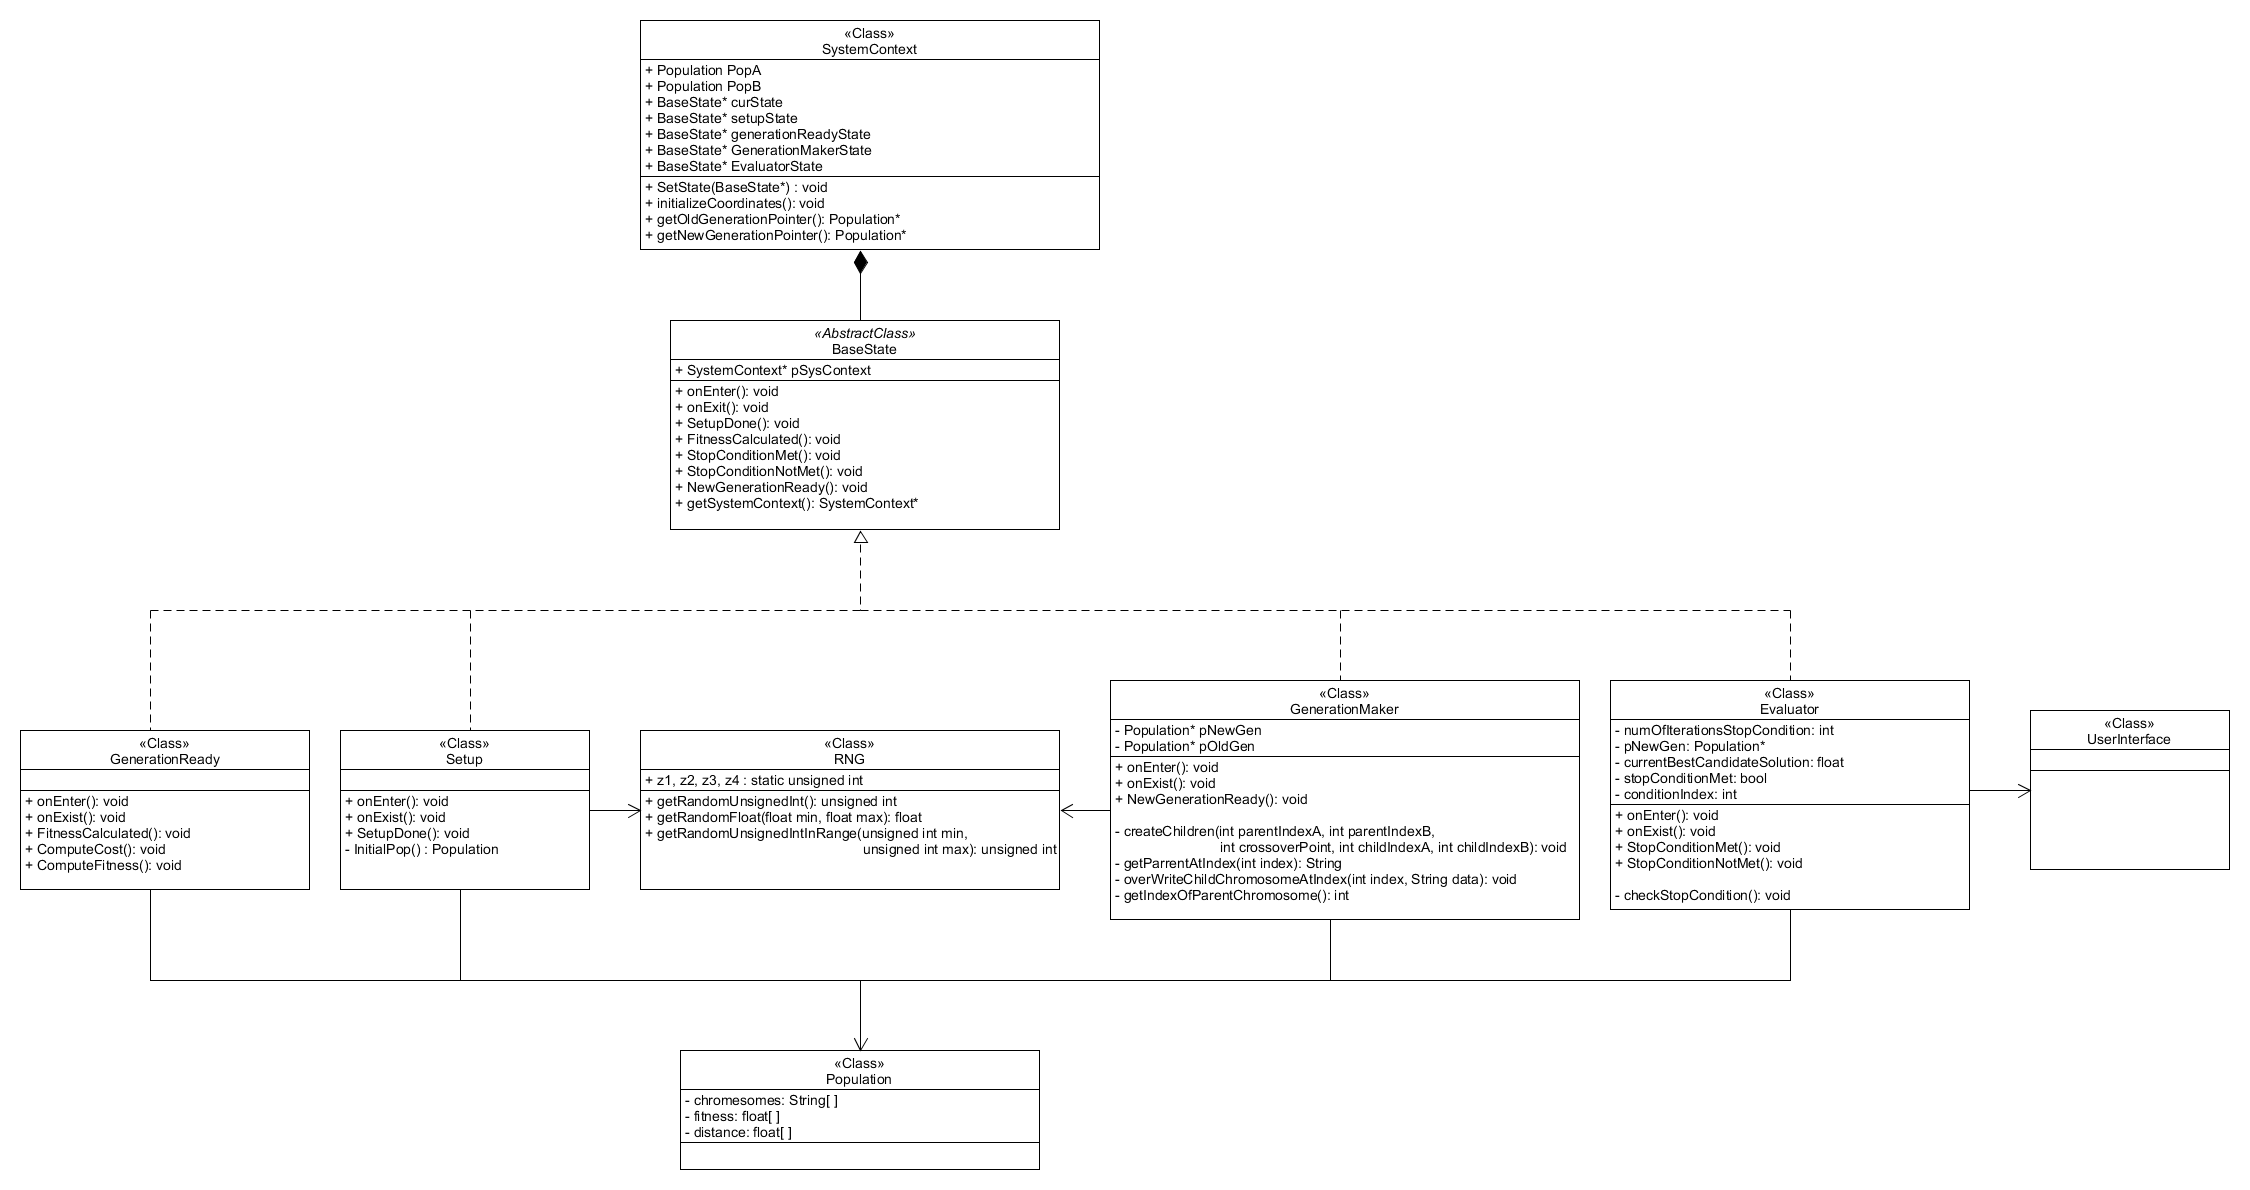
\includegraphics[width=\textwidth]{Images/ClassDiagram.PNG}}\\[0.5cm]
	\caption{Class diagram for the developed system.}
	\label{fig:ClassDiagram}
\end{figure}

As mentioned in the Design chapter a State Machine pattern has been chosen as a good fit for this system and a \textbf{SystemContext} class has been made to handle the holding and switching of states. The abstract class \textbf{Statebase} has virtual methods of each event needed for switching between states. Because StateBase is abstract each state class that inherits from the class needs to implement the corresponding method for changing state. I.e GenerationReady needs to implement FitnessCalculated() otherwise a default version will be called and an exception is called.

The four states functionality is described under the design chapter and can be summed up to:

\begin{itemize}
	\item \textbf{Setup}: Create initial population
	\item \textbf{GenerationReady}: Calculate distance and fitness of population
	\item \textbf{Evaluator}: Checks if there's been generated a better candidate solution, if not increment a counter. If this counter reaches a certain value, our stop condition is met and the program ends.
	\item \textbf{GenerationMaker}: Generate new population by taking the best of the population and use them as parents.
\end{itemize}


\subsection{Timer}
One of the requirements for this assignment was to implement and test a part of the systems functionality on the ZYBO-board. So, different functionalities of the system were timed to examine what functionality of the system is most time consuming. To time the different functionalities a TimerClass was implemented. The class diagram for the TimerClass can be seen on \cref{fig:TimerClass_CD}. The library \textbf{XScuTimer.h} were used. 
\begin{figure}[H]
	\centering
	{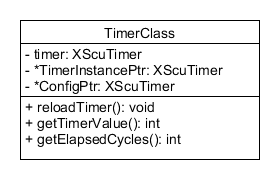
\includegraphics[width=\textwidth/2]{Images/TimerClass_CD.PNG}}\\[0.5cm]
	\caption{Class diagram for the TimerClass.}
	\label{fig:TimerClass_CD}
\end{figure}

The idea was to measure the most time consuming functionality in the system and hardware accelerate that functionality on the ZYBO-board and test the improvement. Three functionalities were time; the calculation of distance for each population, the calculation of fitness for each population and the generation of a new generation. Each of the functionalities were timed five times and the were mean calculated. On \cref{fig:timing_barGraph} a bar-graph of the timing results are presented. 

\begin{figure}[H]
	\centering
	{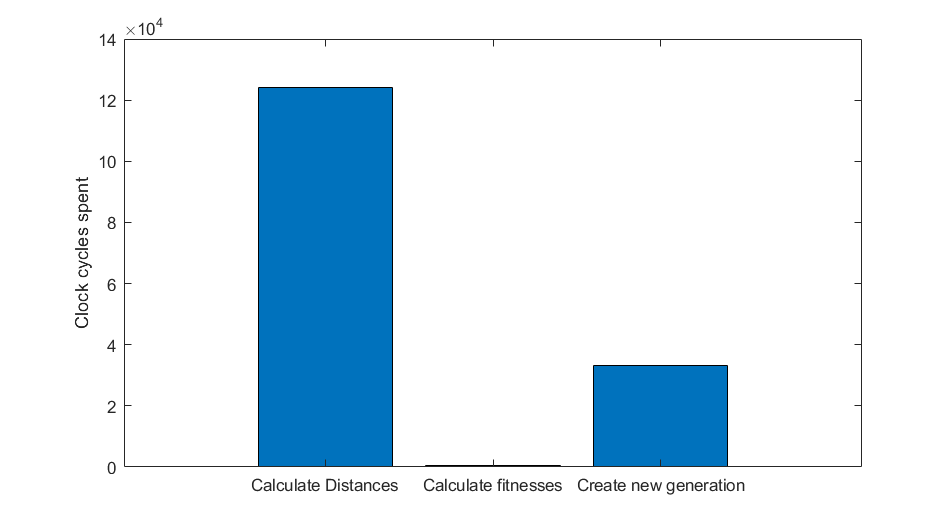
\includegraphics[width=\textwidth]{Images/timing_barGraph.png}}\\[0.5cm]
	\caption{Timing of functionalities bar-graph}
	\label{fig:timing_barGraph}
\end{figure}

Its clear that the calculation of distances is the most time consuming functionality. So, this functionality will be hardware accelerated on the ZYBO-board.


\section{Test of system}
10 predetermined coordinates has been hardcoded into the program. The setup class makes an initial population each with these 10 coordinates in a random order. The population is evaluated and a new population is made based on the best performing of the population. Whenever a new better solution(population) is found, this is saved as the best so far. If no better solution is found after 19 iteration, the program stops and the best solution has been found. An example of this can be seen below on \cref{fig:algo_test_sw}.

\begin{figure}[H]
	\centering
	{\includegraphics[width=\textwidth/2]{Images/algo_test_sw.png}}\\[0.5cm]
	\caption{Test of genetic algorithm}
	\label{fig:algo_test_sw}
\end{figure}

\section{SystemC}

